\documentclass[12pt]{revtex4}
\usepackage{graphicx,amsmath}
\usepackage{dcolumn}% Align table columns on decimal point
\usepackage{bm}% bold math


\begin{document}
\title{POWER DISSIPATED IN A DOUBLE CURRENT-LOOP SYSTEM}
\author{Cristian Alonso Heredia}
\email{cristianheredia@gmail.com}

\affiliation{PHYSICS DEPARTMENT CALIFORNIA STATE
UNIVERSITY, SAN FRANCISCO}

\date{March 19, 2008}
\begin{abstract}
We explore three different methods to find the power dissipated in a two current-loop system.
\end{abstract}
\maketitle

\section{Magnetic fields do no work}

The main motivation for the project is the postulate: magnetic fields due no work. Although not very intuitive, it can easily be shown that for a charged particle displaced by a magnetic field, the work contribution due to the magnetic field is zero. 

\begin{eqnarray}
dW_{mag} &=& \label{eqn:work} \vec{F} \cdot  \vec{dl}\\ \nonumber
&=& q(\vec{v} \times \vec{B}) \cdot \vec{dl} \\  \nonumber
&=& q(\vec{v} \times \vec{B}) \cdot \vec{v}dt\\ \nonumber
&=&0
\end{eqnarray}


However, the above derivation does not lend itself well to all scenarios. For example, imagine a simple two bar magnet system. Picture the two magnets, magnet A and magnet B, held closely together, with like poles facing.  In this scenario the bar magnets are repelling each other.  If magnet A were released it would fly away from magnet B.  Which raises the question: What is doing the work to displace the magnet? Certainly there must be magnetic fields at work: The underlying forces doing the work must be electric. \\


We will try to understand the underlying physics involved by observing forces and work done by displacing one loop in a two current-loop system; we do this by holding one loop fixed and allowing the other to move.  
\subsection{Magnetic force on a current carrying wire}

\begin{equation}
\vec{F}=\int I (\vec{dl} \times \vec{B}) \label{eqn:fwire}
\end{equation}

 \begin{figure}[h]
\begin{center}
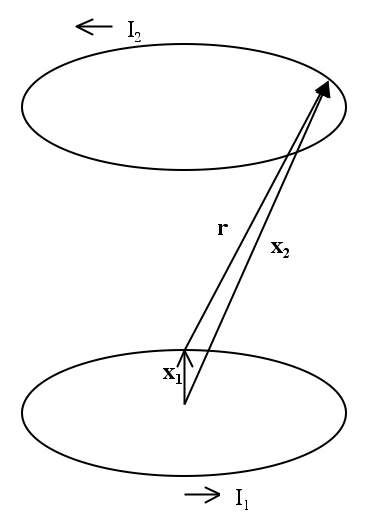
\includegraphics[width=0.5\textwidth]{rx.png} 
\end{center}
\caption{\label{fig:rx} The loop with current $I_1$ is held fixed.  $x_1$ extends from the origin, center of loop 1, and lives in the plane of the loop.}
\end{figure}      

For FIG. (\ref{fig:rx}) $\vec{r}=\vec{x_2}-\vec{x_1}$, $r=| \vec{x_1}-\vec{x_2}|$, and 

\begin{equation}
\frac{\vec{x_2}-\vec{x_1}}{| \vec{x_2}-\vec{x_1}|^3}=-\nabla_2 \frac{1}{| \vec{x_2}-\vec{x_1}|}  \label{eqn:negdel}
\end{equation}
\\
From Eq. (\ref{eqn:fwire}) and using the Biot-Savart law for the magnetic field due to a current carrying wire

\begin{equation}
\vec{B}=\frac{\mu_{0}I}{4\pi} \int \frac{\vec{dl} \times \hat{r}}{r^{2}} \label{eqn:biot}
\end{equation}
the force on one loop due to another is 

\begin{eqnarray*}
\vec{F}_{21}&=&\oint I_{2} (\vec{dl_{2}} \times \vec{B_{1}})\\  \\ 
&=&I_{2} \oint (\vec{dl_{2}} \times \frac{\mu_{0}I_{1}}{4\pi} \oint \frac{\vec{dl_{1}} \times \hat{r}}{r^{2}})\\  \\ 
&=&\frac{\mu_{0}I_{1}I_{2}  }{4\pi} \oint \oint \left[\vec{dl_{2}} \times  \frac{(\vec{dl_{1}} \times \hat{r})}{r^{2}}\right]\\  \\
\end{eqnarray*}

invoking the BAC CAB vector relationship and applying Eq. (\ref{eqn:negdel})
\begin{eqnarray*} 
&=&\frac{\mu_{0}I_{1}I_{2}  }{4\pi} \oint \oint \left[\vec{dl_{1}}(\vec{dl_{2}} \cdot \frac{\hat{r}}{r^{2}})-\frac{\hat{r}}{r^{2}}(\vec{dl_{2}} \cdot \vec{dl_{1}})\right]\\  \\ 
&=&\frac{\mu_{0}I_{1}I_{2}  }{4\pi} \oint \oint \left[ \vec{dl_{1}}(-\vec{dl_{2}} \cdot \nabla_2( \frac{1}{r}))-\frac{\hat{r}}{r^{2}}(\vec{dl_{2}} \cdot \vec{dl_{1}}) \right] \\  \\ 
\end{eqnarray*}
At this juncture we take advantage of the fundamental theorem for gradients
\begin{eqnarray*}
\int_{a}^{b} \nabla F \cdot \vec{dl}=F(b)-F(a)
\end{eqnarray*}
Conveniently we are dealing with two closed loops; for closed loops the end points are the same. 
\begin{eqnarray*}
\oint \nabla F \cdot \vec{dl}=0
\end{eqnarray*}

Hence, the force simplifies to 
\begin{equation}
F_{12}=- \frac{\mu_{0} I_{1}I_{2}}{4\pi} \oint \oint \frac{\hat{r}}{r^{2}}  \vec{dl}_{1} \cdot \vec{dl}_{2}\label{eqn:forceloop}
\end{equation}

$\vec{F}_{12}=-\vec{F}_{21}$ since $\hat{r}$ changes direction.







\section{Energy}

Potential energy for a dipole moment in a magnetic field 

\begin{equation}
\label{potential }
U=-\vec{m} \cdot \vec{B}
\end{equation}

where 

\begin{equation}
\label{dipole}
\vec{m} =\int I \vec{da}
\end{equation}

Thus, the force on an infinitesimal loop with magnetic dipole moment $\vec{m}$, in a magnetic field $\vec{B}$ is 

\begin{equation}
\label{eqn:Uforce}
\vec{F}=\nabla (\vec{m} \cdot \vec{B})
\end{equation}

This is an interesting equation.  Generally to solve for work when given a force one simply follows the regimen given in equation 1.  Naively substituting Eq. (\ref{eqn:Uforce}) into Eq. (\ref{eqn:work}) we have 
\begin{equation}
\label{eqn:dwork}
dw=\nabla (\vec{m} \cdot \vec{B}) \cdot \vec{dl}
\end{equation}


Alas, we have work being done by a magnetic field.  We're in a bit of a predicament here. Ostensibly the above quantity describes the work being done by the magnetic field. However, the means by which we arrived at work is not necessarily correct. 


\newpage
\section{solving for power in the two current-loop system}
In order to understand the work being done we will further examine the power in the two-loop system using three different methods.  In each case we will begin by presenting a diagram of the system, then the pertinent coordinate system, as well as the relevant binomial expansion of the vector describing the relative distance between the current loops, and finally the power of the system.  


\subsection{Determining power in two loop system via potential energy, P= $\vec{F_{U}} \cdot \vec{v}$= $\nabla (\vec{m_2} \cdot \vec{B_1}) \cdot \vec{v}$}

\begin{figure}[h]
\begin{center}
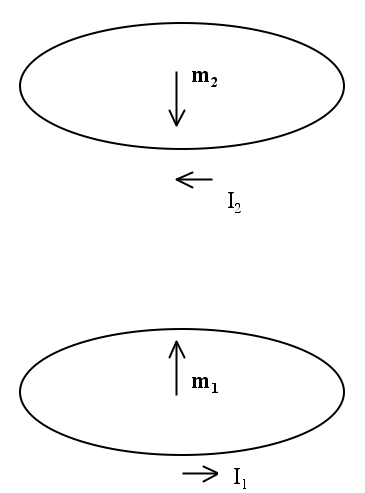
\includegraphics[width=0.5\textwidth]{mm.png} 
\end{center}
\caption{\label{fig:2loop} Two loop current system where the origin is at the center of the first loop.  Since the currents are in opposite directions the two loops repel each other. 
}
\end{figure}      

\subsubsection{Coordinate System}
For this system Cartesian coordinates were used. 

\subsubsection{Binomial Expansion}\label{bin.mU}
For z$\gg$a
\begin{eqnarray*}
\left(a^2+z^2\right)^{-5/2}&=&\left(a^2+z^2\right)^{-5/2}\\
&=&\frac{1}{z^5}\left(1+(\frac{a}{z})^2\right)^{-5/2}\\
&\simeq& \frac{1}{z^5}\left(1-\frac{5}{2}(\frac{a}{z})^2+...\right)\\
&\simeq& \frac{1}{z^5}\\
\end{eqnarray*}

\subsubsection{Power}
\begin{eqnarray*}
P&=&\vec{F_{U}} \cdot \vec{v}\\
&=&\nabla (\vec{m_2} \cdot \vec{B_1}) \cdot \vec{v}\\
\end{eqnarray*}
The vector $\vec{v}$ is the velocity of the moving loop; $\vec{F_{U}} $ is the force found by taking the gradient of the potential, Eq. (\ref{eqn:Uforce});  $\vec{m_2}$ is the magnetic moment of the second loop.\\    \\ 
Using the Biot-Savart Law, Eq. (\ref{eqn:biot}), we evaluate the magnetic field at the center of loop 2 
\begin{equation}
\vec{B_1}=\frac{\mu_{0}I_2}{2} \frac{a^2}{\left(a^2+z^2\right)^{3/2}} \label{eqn:bz} \hat{z}
\end{equation}


Now, 
\begin{eqnarray*}
P&=&\nabla (I_2 \pi a^2 \hat{z}\cdot \vec{B_1}) \cdot \vec{v}\\
&=&\nabla (I_2 \pi a^2 \hat{z}\cdot \frac{\mu_{0}I_1}{2} \frac{-a^2}{\left(a^2+z^2\right)^{3/2}} \label{eqn:bz} \hat{z}) \cdot \vec{v}\\
&=& \frac{-\mu_{0}I_1 I_2a^4}{2}\nabla \left(  \frac{1}{\left(a^2+z^2\right)^{3/2}} \right) \cdot \vec{v}\\
&=& \frac{-\mu_{0}I_1 I_2a^4}{2} \left(  \frac{-3 z }{\left(a^2+z^2\right)^{5/2}} \hat{z}\right) \cdot \frac{dz}{dt}\hat{z}\\
&=& \frac{\mu_{0}I_1 I_2a^4}{2} \left(  \frac{3 z }{\left(a^2+z^2\right)^{5/2}} \hat{z}\right) \cdot \frac{dz}{dt}\hat{z}\\
\end{eqnarray*}

Applying the binomial expansion, Section \ref{bin.mU}.                                                                                                                             
\begin{eqnarray}
P&\simeq&\frac{\mu_{0}I_1 I_2a^4}{2} \frac{3 z }{z^5}  \frac{dz}{dt}\\ \nonumber
&=& \frac{3\mu_{0} I_{1}I_{2}\pi}{2} \Big\{\frac{a}{z}\Big\}^{4}\frac{dz}{dt}
\end{eqnarray}

    
\newpage
\subsection{Power in loop 2  due to loop 1 using P=$\vec{F_{21}} \cdot \vec{v}$}
The vector $\vec{v}$ is the relative velocity of the loops in the z direction,  and $\vec{F_{21}} $ is the force due to a current carrying wire. 

\begin{figure}[h]
\begin{center}
\includegraphics[width=0.5\textwidth]{basicsetup.jpg} 
\end{center}
\caption{\label{fig:2loop} Two loop current system where the origin is at the center of the first loop.}
\end{figure}      

\subsubsection{Coordinate System}
Using Cartesian coordinates:
\begin{eqnarray*}
\vec{r}&=&(x_{2}-x_{1})\hat{x}+(y_{2}-y_{1})\hat{y}+z\hat{z}\\
&=&a(\cos\phi_{2}-\cos\phi_{1})\hat{x}+a(\sin\phi_{2}-\sin\phi_{1})\hat{y}+z\hat{z}\\
\end{eqnarray*}

\begin{eqnarray*}
r^{2}=&&\vec{r} \cdot \vec{r}\\
=&&a^{2}(\cos^{2}\phi_{2} +\cos^{2}\phi_{1}-2\cos\phi_{2}\cos\phi_{1})\\
 &&+a^{2}(\sin^{2}\phi_{2}+\sin^{2}\phi_{1}-2\sin\phi_{2}\sin\phi_{1})+z^{2}\\
 =&&z^{2}+2a^{2}-2a^{2}(\cos\phi_{2}\cos\phi_{1}+\sin\phi_{2}\sin\phi_{1})\\
  =&&z^{2}+2a^{2}-2a^{2}(\cos(\phi_{2}-\phi_{1})\\
  =&&z^{2}+2a^{2}[1-(\cos(\phi_{2}-\phi_{1})]
\end{eqnarray*}

\subsubsection{Binomial Expansion}\label{bin}

\begin{eqnarray*}
&&[z^{2}+2a^{2}(1-\cos(\phi_{2}-\phi_{1})]^{-3/2} \\ \\
&&=\frac{1}{z^{3}}[1+2\big\{ \frac{a}{z}\big\}^{2}(1-\cos(\phi_{2}-\phi_{1})]^{-3/2} \\ \\
&&\simeq \frac{1}{z^{3}}[1-3\big\{ \frac{a}{z}\big\}^{2}(1-\cos(\phi_{2}-\phi_{1})+...] 
\end{eqnarray*}

\subsubsection{Power}

\begin{eqnarray*}
P&=&\vec{F_{21}} \cdot \vec{v}\\ \\
&=&- \frac{\mu_{0} I_{1}I_{2}}{4\pi} \oint \oint (\frac{\hat{r}}{r^{2}}  \vec{dl}_{1} \cdot \vec{dl}_{2}) \cdot  \vec{v}\\ \\
&=&- \frac{\mu_{0} I_{1}I_{2}}{4\pi} \oint \oint (\frac{\hat{r}}{r^{2}}  \vec{dl}_{1} \cdot \vec{dl}_{2}) \cdot  \frac{d\vec{z}}{dt}\\ \\
&=&- \frac{\mu_{0} I_{1}I_{2}}{4\pi} \oint \oint ( \vec{dl}_{1} \cdot \vec{dl}_{2}) \frac{\vec{r}}{r^{3}} \cdot  \hat{z}\frac{dz}{dt}\\ \\
&=&- \frac{\mu_{0} I_{1}I_{2}}{4\pi} \oint \oint ( \vec{dl}_{1} \cdot \vec{dl}_{2}) \frac{z}{r^{3}} \frac{dz}{dt}\\ \\
&=&- \frac{\mu_{0} I_{1}I_{2}z}{4\pi} \frac{dz}{dt} \oint \oint ( \vec{dl}_{1} \cdot \vec{dl}_{2}) \frac{1}{r^{3}} \\ \\
&=&- \frac{\mu_{0} I_{1}I_{2}z}{4\pi} \frac{dz}{dt} \oint \oint {dl}_{1} {dl}_{2}\cos(\phi_{2}-\phi_{1}) \frac{1}{r^{3}} \\ \\
&=&- \frac{\mu_{0} I_{1}I_{2}z}{4\pi} \frac{dz}{dt} \oint  \oint \frac{{dl}_{1} {dl}_{2}\cos(\phi_{2}-\phi_{1})} {[z^{2}+2a^{2}(1-(\cos(\phi_{2}-\phi_{1}))]^{3/2}} \\ \\
\end{eqnarray*}

The magnitude of $\vec{r}$ is rewritten using the expression found above.  In order to ease the solving of the integral we can take the binomial expansion of the denominator, assuming $z\gg a$.  We begin by factoring out $\frac{1}{z^3}$, see Section \ref{bin}.



Now,
\begin{eqnarray*}
P &=&\vec{F_{21}} \cdot \vec{v}\\ 
&=&- \frac{\mu_{0} I_{1}I_{2}}{4\pi z^{2}} \frac{dz}{dt} \oint  \oint dl_{1} dl_{2} \cos(\phi_{2}-\phi_{1})  \left[1-3\big\{ \frac{a}{z}\big\}^{2}\left(1-\cos(\phi_{2}-\phi_{1})\right) \right] \\ \\
\end{eqnarray*}
Observing, over the integration range $0$ to $2\pi$,  the only terms that survive are those with $\cos^2{\theta}$ terms.  We can also rewrite $dl$ in terms of $a$ and $d\phi$.
\begin{eqnarray*}
&=&- \frac{\mu_{0} I_{1}I_{2}a^{2}}{4\pi z^{2}} \frac{dz}{dt} \oint  \oint d\phi_{1} d\phi_{2} \cos(\phi_{2}-\phi_{1})  [1-3\big\{ \frac{a}{z}\big\}^{2}(1-(\cos(\phi_{2}-\phi_{1}))] \\ \\
&=&- \frac{\mu_{0} I_{1}I_{2}a^{2}}{4\pi z^{2}} \frac{dz}{dt} \oint d\phi_{2}3\big\{ \frac{a}{z}\big\}^{2}\pi \\ \\
&=&- \frac{3\mu_{0} I_{1}I_{2}a^{4}}{4 z^{4}} \frac{dz}{dt} \oint d\phi_{2}\\ \\ 
&=&- \frac{3\mu_{0} I_{1}I_{2}\pi}{2} \Big\{\frac{a}{z}\Big\}^{4}\frac{dz}{dt}
\end{eqnarray*}


\subsection{Work done on loop 1 by loop 2 using P=$IV$}

By moving loop 2 in the positive z direction an emf, $V_{21}$, is induced in loop 1. 

\begin{figure}[h]
\begin{center}
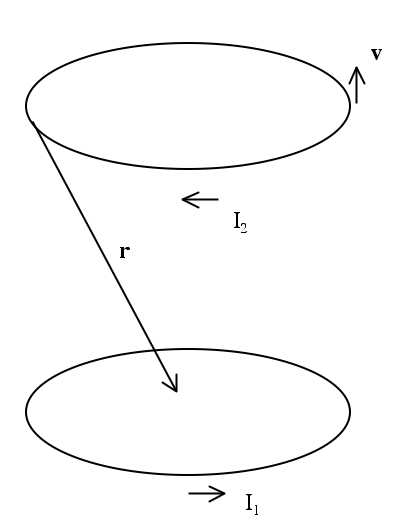
\includegraphics[width=0.5\textwidth]{rext.png} 
\end{center}
\caption{\label{fig:2loop} The vector $\vec{r}$ extends from loop 2 and sweeps the area enclosed by loop 1.}
\end{figure}    


\subsubsection{Coordinate System}
Using polar coordinates:
\begin{eqnarray*}
r^{2}=&&\vec{r} \cdot \vec{r}\\
=&&a^{2}+\rho_{1}^2+z^{2}-2 a \rho_{1} \cos(\phi_{2} - \phi_{1})\\
\end{eqnarray*}

\subsubsection{Binomial Expansion}\label{bin.IV}
Once again soliciting the binomial expansion we arrive at 
\begin{eqnarray*}
\frac{1}{r}=&&\frac{1}{z}\left[1+\frac{a^2+\rho_{1}^2}{z^2}-\frac{2a\rho_{1}}{z} \cos(\phi_{2} - \phi_{1})\right]^{-1/2}\\
=&&\frac{1}{z}\left[1-\frac{a^2+\rho_{1}^2}{2 z^2}+\frac{a\rho_{1}}{z^2} \cos(\phi_{2} - \phi_{1})+...\right]\\
\approx&&\frac{1}{z}-\frac{a^2+\rho_{1}^2}{2 z^3}+\frac{a\rho_{1}}{z^3} \cos(\phi_{2} - \phi_{1})
\end{eqnarray*}

\subsubsection{Power}

\begin{eqnarray*}
P&=&I_{1}V_{21}\\ \\
\end{eqnarray*}
Invoking Maxwell's equations we begin to express the power in terms of currents. 
\begin{eqnarray*}
P&=&-I_{1} \oint \vec{E}_{ind} \cdot \vec{dl}_{1} \\ \\
&=&I_{1} \frac{d}{dt}\int \vec{B}_{2} \cdot \vec{da}_{1} \\ \\
&=&I_{1} \frac{d}{dt}\int \frac{\mu_{0}I_{2}}{4\pi} \int \frac{\vec{dl}_{2} \times \hat{r}}{r^{2}} \cdot \vec{da}_{1} \\ \\
&=&\frac{\mu_{0}I_{1}I_{2}}{4\pi} \frac{d}{dt}\int \int \frac{\vec{dl}_{2} \times \hat{r}}{r^{2}} \cdot \vec{da}_{1} \\ \\
&=&\frac{-\mu_{0}I_{1}I_{2}}{4\pi} \frac{d}{dt}\int  \oint  \int \frac{\vec{dl}_{2} \times \hat{r}}{r^{2}} \cdot \rho_{1} d\rho_{1} d\phi_{1} \hat{z}\\ \\
&=&\frac{\mu_{0}I_{1}I_{2}}{4\pi} \frac{d}{dt}\int  \oint \int \vec{dl}_{2} \times \nabla_1( \frac{1}{r}) \cdot \rho_{1} d\rho_{1} d\phi_{1} \hat{z}\\ \\
&=&\frac{\mu_{0}I_{1}I_{2}}{4\pi} \frac{d}{dt}\int  \oint \int a d\phi_{2} \hat{\phi}_{2} \times \nabla_1( \frac{1}{r}) \cdot \rho_{1} d\rho_{1} d\phi_{1} \hat{z}\\ \\
&=&\frac{\mu_{0}I_{1}I_{2}}{4\pi} \frac{d}{dt}\int  \oint \oint a d\phi_{2}(\hat{z}\times \hat{\phi}_{2} ) \cdot \nabla_1( \frac{1}{r})  \rho_{1} d\rho_{1} d\phi_{1} \\ \\
&=&\frac{\mu_{0}I_{1}I_{2}}{4\pi} \frac{d}{dt}\int  \oint \oint a d\phi_{2} \hat{\rho_{2}} \cdot \nabla_{1}( \frac{1}{r})  \rho_{1} d\rho_{1} d\phi_{1} \\ \\
\end{eqnarray*}

From the diagram

\begin{equation}
\hat{\rho_2}=\hat{\rho_1}\cos(\phi_{2}-\phi_{1})+\hat{\phi_1}\sin(\phi_{2}-\phi_{1})
\end{equation}

and

\begin{equation}
\hat{\rho_2} \cdot \nabla_{1}=\cos(\phi_{2}-\phi_{1})\frac{\partial}{\partial \rho_1}+\sin(\phi_{2}-\phi_{1})\frac{1}{\rho_1}\frac{\partial}{\partial \phi_1}
\end{equation}


Now, 
\begin{eqnarray*}
P=\frac{a \mu_{0}I_{1}I_{2}}{4\pi} \frac{d}{dt}\int  \oint \oint  d\phi_{2} \left( \cos(\phi_{2}-\phi_{1})\frac{\partial}{\partial \rho_1}+\sin(\phi_{2}-\phi_{1})\frac{1}{\rho_1}\frac{\partial}{\partial \phi_1} \right)( \frac{1}{r})  \rho_{1} d\rho_{1} d\phi_{1} 
\end{eqnarray*}


Looking at the expression for $\frac{1}{r}$ (\ref{bin.IV}) only the square trigonometric functions survive the closed loop integrals. 
\\ \\
In order to simplify this integral it will be split up into two terms and set the constants and time derivative equal to $C_1$. 

\begin{eqnarray*}
Integral_1&=&C_1\int \oint \oint   \frac{a\rho_{1}}{z^3} \cos^{2}(\phi_{2} - \phi_{1}) d\rho_{1} d\phi_{1} d\phi_{2} \\ \\
&=&C_1\oint  \oint    \frac{a^3}{2z^3} \cos^{2}(\phi_{2} - \phi_{1})  d\phi_{1} d\phi_{2} \\ \\
&=&\oint \frac{a^3 \pi}{2z^3} d\phi_{2} \\ \\
&=&C_1\frac{ a^3 \pi^2}{z^3}  \\ \\
\end{eqnarray*}

\begin{eqnarray*}
Integral_2&=&C_1\int \oint \oint   \frac{a \rho_{1}}{z^3} \sin^{2}(\phi_{2} - \phi_{1}) d\rho_{1} d\phi_{1} d\phi_{2} \\ \\
&=&C_1 \oint \oint   \frac{a^3}{2z^3} \sin^{2}(\phi_{2} - \phi_{1})d\phi_{2}  d\phi_{1}  \\ \\
&=&C_1\oint \frac{a^3\pi}{2z^3}   d\phi_{1}  \\ \\
&=&C_1\frac{ a^3 \pi^2}{z^3}  \\ \\
\end{eqnarray*}

Combining the results yields

\begin{eqnarray*}
P&=&C_1\frac{ 2a^3 \pi^2}{z^3}  \\ \\
&=&\frac{a\mu_{0}I_{1}I_{2}}{4\pi} \frac{d}{dt} \frac{ 2a^3 \pi^2}{z^3} \\ \\
&=&\frac{\mu_{0}I_{1}I_{2}}{2}  \frac{ -3a^4 \pi}{z^4} \frac{dz}{dt}\\ \\
&=&- \frac{3\mu_{0} I_{1}I_{2}\pi}{2} \Big\{\frac{a}{z}\Big\}^{4}\frac{dz}{dt}
\end{eqnarray*}


In moving loop 2 an emf was induced on loop 1.  However, since $\frac{dz}{dt}$ is a relative velocity, an emf is also induced in loop 2 by loop 1. Thus, the work done on loop 1 by loop 2 is twice that calculated for the one loop. 
\begin{equation}
P=  - 3\mu_{0} I_{1}I_{2}\pi\Big\{\frac{a}{z}\Big\}^{4}\frac{dz}{dt} \label{eqn:totalpower}
\end{equation}

\section{Apparatus}
\section{Experimental Data}


\section{Conclusion}
So in summary we used $P=\nabla (\vec{m_2} \cdot \vec{B_1}) \cdot \vec{v}$, $P= \vec{F_{21}} \cdot \vec{v}$, and $P= IV $ to determine energy in the two loop system.
We know what the magnitude of the work is, Eq (\ref{eqn:dwork}). However, our challenge is to properly describe it, determining how where the Magnetic fields turn into Electric fields in order to do the work.  

\begin{acknowledgements}
Acknowledgement. 
\end{acknowledgements}


\appendix

\section{Supplemental Problems}

\newpage
\begin{thebibliography}{number} 

\bibitem{Griffiths} 
David J. Griffiths, \textit{Introduction to Electrodynamics 3rd. Edition} (Prentice Hall, Upper Saddle River, New Jersey 1999)\\
\bibitem{jackson}
J.D. Jackson, \textit{Classical Electrodynamics 3rd. Edition} (John Wiley $\&$ Sons, New York 1999)\\
\bibitem{Magnetism}
Mathias Getzlaff, \textit{Fundamentals of Magnetism} (Springer, New York 2008)\\
\bibitem{lea}
Susan M.  Lea, \textit{Mathematics For Physicists} (Brooks/Cole, Belmont, CA 2004) \\
\bibitem{GandR}
I.S. Gradshteyn and I.M. Ryzhik , \textit{Table of Integrals, Series, and Products} (Academic Press; 4th edition 1965)




\end{thebibliography}


\end{document}


